% document classes: article, report, letter, book, proc, slides

\documentclass[11pt]{article}
\usepackage[left=1cm, right=1cm, marginparwidth=1cm, marginparsep=3mm]{geometry}
\geometry{a4paper}                   % ... or a4paper or a5paper or ... 

%\geometry{landscape}                % Activate for for rotated page geometry
%\usepackage[parfill]{parskip}    % Activate to begin paragraphs with an empty line rather than an indent
\usepackage{graphicx}
\usepackage{wrapfig}
\usepackage{amssymb}
\usepackage{epstopdf}
\usepackage{marginnote}
\usepackage{datetime}
\usepackage{pdflscape}
\newcounter{notes}

% taken from: http://www.latex-community.org/forum/viewtopic.php?f=44&t=11761
\newcommand{\nummarginnote}[1]{
	\refstepcounter{notes}
	\marginpar{\textsuperscript{\thenotes}\footnotesize{#1}}
}

\DeclareGraphicsRule{.tif}{png}{.png}{`convert #1 `dirname #1`/`basename #1 .tif`.png}


\begin{document}

\pagenumbering{gobble}
\begin{landscape}
\begin{center}
\vfill
\huge{A sample presentation}
\hrule\vspace{0.5cm}
\vfill
Landscape slide
\vfill
Bottom of the page
\end{center}
\end{landscape}


\pagenumbering{arabic}
\begin{wrapfigure}{o}{0.5\textwidth}
	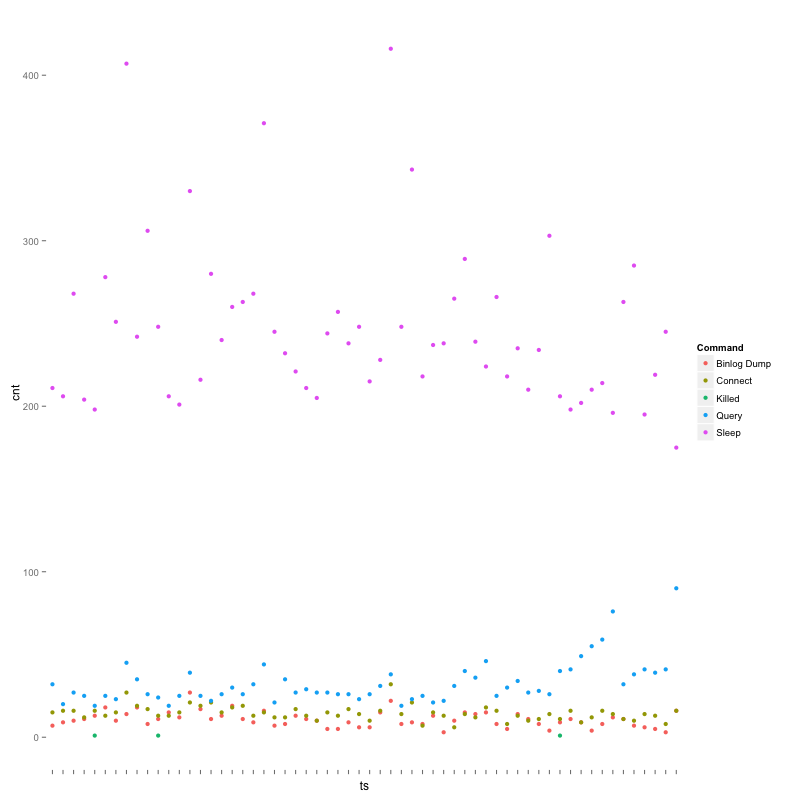
\includegraphics[width=0.5\textwidth]{./images/genplot.png}
   \caption{sample graphic}
\end{wrapfigure}

This is a test idea for sharing slides for a presentation along with a text representing a possible version of the presentation content\footnote{These may be completed after a presentation is delivered; the portrait pages would serve the same purpose as a recording}.

\pagebreak
Page 2


\pagebreak
Page 3


\pagebreak

\pagenumbering{gobble}
\begin{landscape}
  \begin{center}
    Second slide
  \end{center}
\end{landscape}


%\section{}
%\subsection{}



\end{document}  
